% Teilauswertung 2

\newpage
\section{Rotationsgeschwindigkeitsabhängigkeit von Schichtdicken}
\label{sec:rot}

In diesem Abschnitt wird die Abhängigkeit der Schichtdicke $d$ von der Rotationsgeschwindigkeit $\omega$ betrachtet. Dafür wird die \textit{Schubert-Gleichung} zum fitten der Messwerte benutzt und ist gegeben durch:
\begin{gather}
    d = A \cdot \left(\frac{1950\,\frac{1}{\mathrm{min}}}{\omega}\right)^{\frac{1}{2}} \cdot \left(\frac{c_0}{20\,\frac{\mathrm{g}}{\mathrm{l}}}\right)\cdot\left(\frac{M_\mathrm{W}}{100\,\frac{\mathrm{kg}}{\mathrm{mol}}}\right)^{\frac{1}{4}}~,
    \label{eq:schubert}
\end{gather}
wobei $c_0$ die Polymerkonzentration der Lösung, $M_\mathrm{W}$ das Molekulargewicht der Lösung und $A$ der Skalierungsfaktor (abhängig von Umgebungsparameter) in Einheiten von nm ist. \cite{Ruderer2009}

Um die Gleichung \ref{eq:schubert} besser zu fitten wird die Polymerkonzentration $c_0$ mit 100\,$\frac{\mathrm{mg}}{\mathrm{mg}}$ und das Molekulargewicht $M_\mathrm{W}$ von 0,217\,$\frac{\mathrm{kg}}{\mathrm{mol}}$ (Chlorbenzol: 0,113\,$\frac{\mathrm{kg}}{\mathrm{mol}}$\cite{MolCB} und Polystyrol: 0,104\,$\frac{\mathrm{kg}}{\mathrm{mol}}$\cite{MolPS}) eingesetzt und zusammen mit dem Wert von 1950\,$\frac{1}{\mathrm{min}}$ umgerechnet in 1950\,rpm\cite{rpminmin} zusammengezogen zur Konstante:
\begin{gather*}
    C = \left(1950\,\mathrm{rpm}\right)^{\frac{1}{2}} \cdot \left(\frac{100\,\frac{\mathrm{g}}{\mathrm{l}}}{20\,\frac{\mathrm{g}}{\mathrm{l}}}\right)\cdot\left(\frac{0,217\,\frac{\mathrm{kg}}{\mathrm{mol}}}{100\,\frac{\mathrm{kg}}{\mathrm{mol}}}\right)^{\frac{1}{4}} %\\[0.2cm]
    \Rightarrow \boxed{C = 47,654\,\mathrm{rpm}^{1/2}}~.
\end{gather*}
Damit vereinfacht sich die \textit{Schubert-Gleichung} zu:
\begin{gather}
    \boxed{d = A \cdot C \cdot \omega^{-1/2}}~.
    \label{eq:schbuertadvanced}
\end{gather}
Der Fit wird wie in Kapitel \ref{sub:fitguete} durchgeführt, wobei wieder  für jede einzelne Messung über die gemessenen Schichtdicken $d$ gemittelt wird. Zusätzlich wird auch die Heterogenität $h$ berechnet, was in Tabelle \ref{tab:rotHetero} nachzulesen ist. Durch den Fit ergeben sich Werte für den Skalierungsfaktor $A$, welche in Tabelle \ref{tab:rot} dargestellt wurden. 
\begin{center}
	\captionsetup{type=table}	
	\begin{tabular}{r | r r | r | r r | r}
                     & \multicolumn{3}{c |}{Reflexion}    & \multicolumn{3}{c}{Tranmission} \\
		$\omega$/rpm & $\langle d \rangle$/\si{\nano\metre} & $d^*$/\si{\nano\metre} & $h$ &$\langle d \rangle$/\si{\nano\metre} & $d^*$/\si{\nano\metre} & $h$ \\
		\hline
         500 & 894.6 & 31.6 &  28.3 & 904.4 & 21.8 &  41.5\\
         750 & 740.5 &  9.0 &  82.3 & 729.1 &  9.7 &  75.2\\
        1000 & 604.6 &  5.9 & 102.5 & 614.6 &  5.0 & 122.9\\
        2000 & 466.7 &  7.5 &  62.2 & 466.2 &  9.2 &  50.7\\
        3000 & 405.2 &  7.9 &  51.3 & 397.2 &  7.4 &  53.7\\
        4000 & 360.8 &  8.2 &  44.0 & 359.4 & 10.3 &  34.9\\
        5000 & 329.7 & 16.4 &  20.1 & 329.7 & 15.8 &  20.9\\
        6000 & 302.7 &  5.8 &  52.2 & 312.1 & 12.3 &  25.4\\
	\end{tabular}
	\captionof{table}{Werte für Heterogenität $h$ bei Reflexion und Transmission}
	\label{tab:rotHetero}
\end{center}
\begin{center}
	\captionsetup{type=table}
	\begin{tabular}{l | c | c }
		  & Reflexion & Tranmission \\
		  \hline
		  $A$/nm & 429.2 & 430.2 \\
	\end{tabular}
	\captionof{table}{Ermittelter Skalierungsfaktor $A$ für Reflexion- und Transmissionsmessung}
	\label{tab:rot}
\end{center}
Weiterhin kann in Abb. \ref{fig:rotation} die Messwerte der Schichtdicke in Abhängigkeit der Rotationsgeschwindigkeit extrapoliert dargestellt. Die Extrapolation wurde hierbei für $\omega \in [0, 10000]\,\mathrm{rpm}$ durchgeführt.
Dabei lässt sich an den Grenzwerten feststellen:
\begin{gather}
    \langle d \rangle \xrightarrow{\omega\rightarrow 0} \infty~~~\langle d \rangle \xrightarrow{\omega\rightarrow \infty} 0~,
\end{gather}
was von einer $y = x^{-1/2}$ Funktion, wie die \textit{Schubert-Gleichung} \ref{eq:schbuertadvanced} eine ist, erwartet wird.
\begin{center}
	\captionsetup{type=figure}
	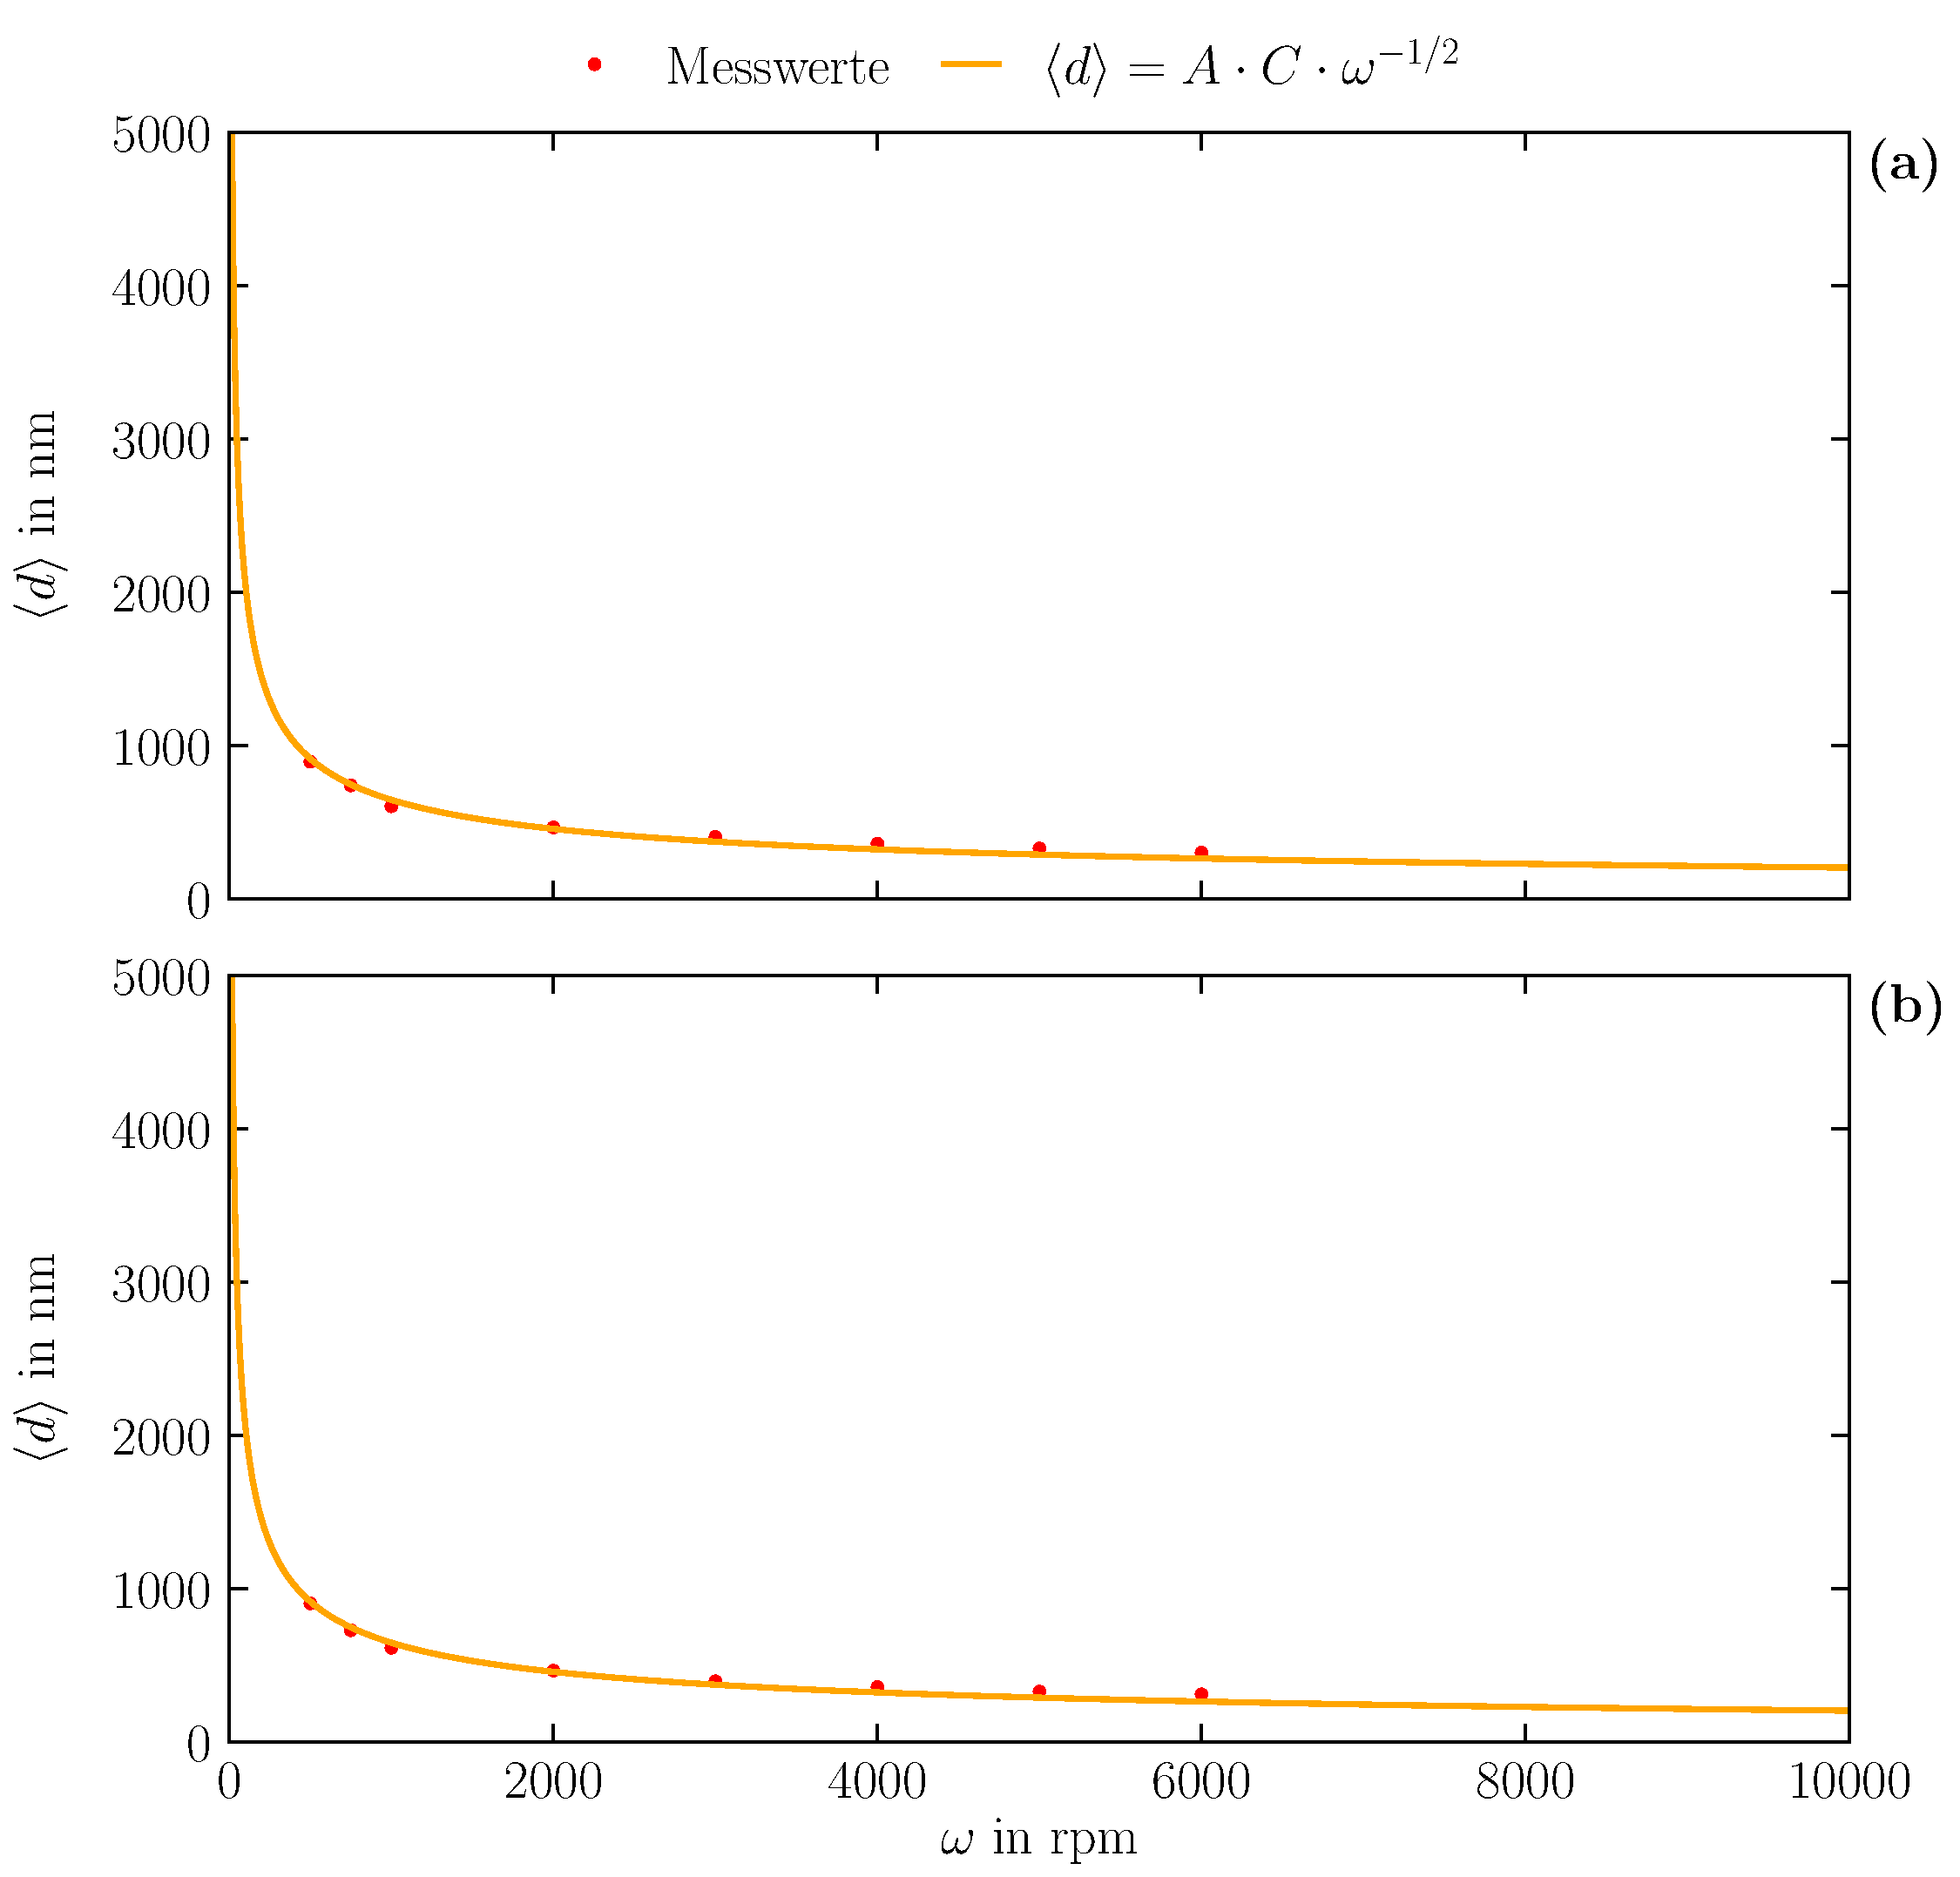
\includegraphics[width=0.9\textwidth]{Auswertung/42/Rotation.pdf}
	\captionof{figure}{Mittelwert der Schichtdicke $\langle d \rangle$ in Abhängigkeit zur Rotationsgeschwindigkeit $\omega$ für Reflexion \textbf{(a)} und Transmission \textbf{(b)} extrapoliert für $\omega \in [0, 10000]\,\mathrm{rpm}$}
	\label{fig:rotation}
\end{center}
Physikalisch ist aber eine Schichtdicke von unendlich weniger sinnvoll, da sich eine endliche Menge von der Lösung auf dem Substart befindet. Es könnte mit genährt eine maximale Schichtdicke angeben, wenn man das Volumen der Lösung auf dem Substrat durch den Flächeninhalt des Substrats teilt. Dies ist aber nicht Teil dieser Arbeit. Zudem ist aber eine unendliche Rotationsgeschwindigkeit genauso nicht physikalisch, da einerseits solche Maschinen nicht existieren,andererseits das Substart bei zu hohen Rotationsgeschwindigkeiten aus der Fassung des Spincoater fliegen kann, was die Probe unbrauchbar macht. Dennoch sind die Messwerte physikalisch richtig, da sich mit höherer Rotationsgeschwindigkeit weniger Lösung auf dem Substart befindet. 

Aus Tabelle \ref{tab:rotHetero} lässt sich auch entnehmen, dass für kleinere Rotationsgeschwindigkeit $\omega$ die Homogenität zunimmt. Es scheint so, dass bei der Heterogenität ein Maximum bei 1000\,rpm erreicht wird, was zur Folge hätte, dass bei \textbf{kleinern und großen} Rotationsgeschwindigkeiten  die Homogenität zunimmt. Dies kann vor allem bei der Transmissionsmessung am deutlichsten erkannt werden. Die Gründe warum die Transmissionsmessung am besten geeignet ist, wurde schon in Kapitel \ref{sub:vergleich} erklärt.